\documentclass[compress]{beamer}

\usetheme{naked}
\usecolortheme{dark}

\usepackage{pgfpages}
\setbeamertemplate{note page}[plain]
\setbeamercolor{note page}{fg=black}
\setbeameroption{show notes on second screen}
%\setbeameroption{hide notes} % Only slides

% \usepackage[utf8]{inputenc} % utf8 file encoding
% \usepackage[UTF8]{ctex}

\usepackage{listings}
\usepackage[T1]{fontenc} % powerful pdf output encoding

\title{Reading and writing flash on GA144}
\date{\today}
\author{James Bowman}

\begin{document}

\titlepage

\begin{wordframe}
\huge
GA144
\note {
\url{http://www.greenarraychips.com/}
}
\end{wordframe}

\begin{imageframe}{GA144}
\end{imageframe}

\begin{frame}
it's a kind of computer
\note{
For a taste of what it's like to program a node:
\tiny
\url{https://mschuldt.github.io/www.colorforth.com/inst.htm}
}
\end{frame}

\begin{imageframe}{simulator}
\note{
This is the arrayForth simulator/IDE

Top right is a picture of the whole chip, 18x8

On the left is the state of the highlighted 8x4 region of CPUs

To the right is a memory dump of one node.

My alternative toolchain is at
\tiny
\url{https://github.com/jamesbowman/ga144tools/blob/master/src/flashwrite.ga}
}
\end{imageframe}

\begin{wordframe} flash
\note{
The GA144 eval board uses a SST25WF080,
an 8 Mbit flash
}
\end{wordframe}

\begin{frame}
it's a kind of memory
\end{frame}

\begin{imageframe}{worker-694267_1920}
\end{imageframe}

\begin{frame}[fragile]
slow to write, slower to erase
\note{
For example, for 4K on SST25W:

\begin{description}
\item[write] .1 ms $(4096 \times 25\mu s)$
\item[erase] 35 ms
\end{description}

On MX25L:

\begin{description}
\item[write] 22.4 ms
\item[erase] 60 ms
\end{description}
}
\end{frame}

\begin{imageframe}{node705}
\note{
The source for node 705's ROM is in block 1428 at
\url{http://excamera.com/files/cf.html}
}
\end{imageframe}

\begin{imageframe}{b1160}
\note{
Chuck's code is at:

\tiny
\url{https://mschuldt.github.io/www.colorforth.com/flash.htm}
}
\end{imageframe}

\begin{imageframe}{sketch}
\note{
A traditional way of managing flash contents.
\begin{itemize}
\item The \textbf{PC} has the original flash image and runs a driver program
\item the microcontroller \textbf{$\mu c$} writes blocks into \textbf{RAM} then copies them to
\textbf{flash}
\end{itemize}
A bootloader is one example of this.

For GA144, there's no microcontroller or RAM.
So must do something different.
}
\end{imageframe}

\begin{wordframe} reading \end{wordframe}

\begin{imageframe}{flashread}
\note{
Node 705 reads the flash, sends the data east.
Node 708 is a UART transmitter.

From the PC's point of view,
it loads the program and the
GA144 dumps the flash contents.

Code is at:

\vspace{10pt}
\tiny

\url{https://github.com/jamesbowman/ga144tools/blob/master/src/flashread.ga}

}
\end{imageframe}

\begin{wordframe} writing \end{wordframe}

\begin{imageframe}{flashread}
\note{
This won't work.
The async node needs to wait for each flash operation.
}
\end{imageframe}

\begin{frame}
need 4K of storage
\note{
But nobody has really figured out how to make an effective large RAM yet.
}
\end{frame}

\begin{imageframe}{1280px-Silent_Reading_time_in_a_Lao_school.jpg}
\LARGE 
RECITE
\vspace{120pt}
\note{
RECITE nodes write out their contents,
then become wire nodes.
}
\end{imageframe}

\begin{imageframe}{flashwrite}
\note{
Code is at
\tiny
\url{https://github.com/jamesbowman/ga144tools/blob/master/src/flashwrite.ga}
}
\end{imageframe}

\begin{frame}[fragile]
\begin{verbatim}
\ Send contents to DST then carry SRC to DST
    @p @p @p @p
      SRC
      DST
      3
      60
    push a! b!
: main
    @+ !b unext
    a!
: wire
    @ !b jump wire
\end{verbatim}
\note{
Each RECITE node uses 3 words for program.
The remaining 61 words of program are available for data.

This is why the constants 3 and 60 (61-1) appear here.

So each node is 122 bytes, and 4K requires 33 nodes.
}
\end{frame}

\begin{imageframe}{flashwrite}
\note{
Nodes 604 through 704 hold 4K of data.

Node 705 erases the flash, then reads from its WEST port to get each word,
and writes it to flash.

After it completes it sends a byte to node 708, which outputs it.
}
\end{imageframe}

\begin{frame}[fragile]
\begin{verbatim}

P=/dev/ttyUSB0

./flash.py $P write war_and_peace.txt

./flash.py $P read new.txt 3359550

\end{verbatim}
\note{
The flash utility is now included in ga144tools

Write speed is about 18K/s
}
\end{frame}

\begin{imageframe}{field-653689_1920.jpg}
\LARGE 
\vspace{120pt}
PLOW
\end{imageframe}

\bgroup
\usebackgroundtemplate{
\tikz[overlay,remember picture] \node[at=(current page.center)] {
   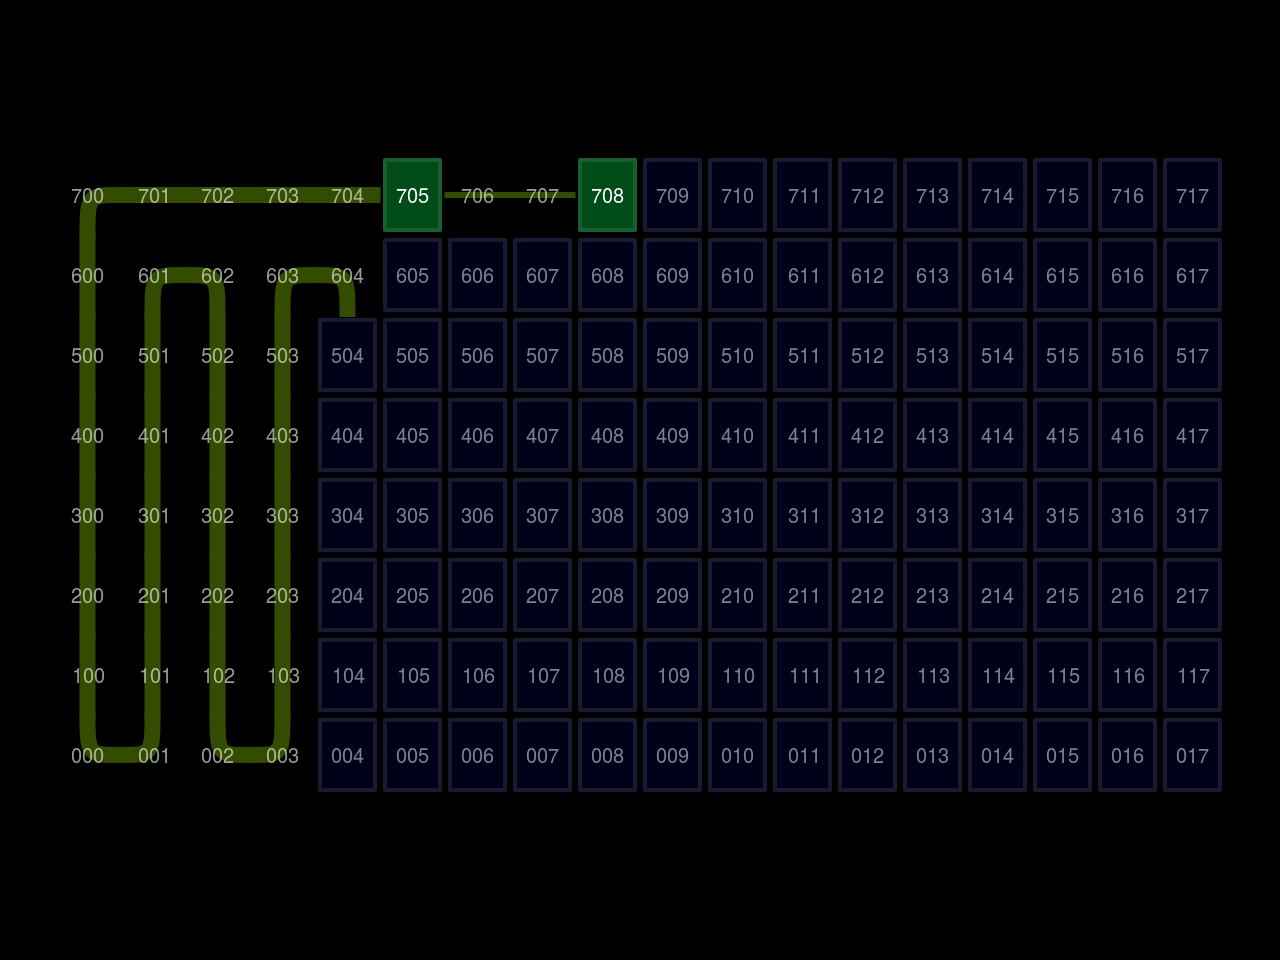
\includegraphics[height=\paperheight,width=\paperwidth]{flashwrite}};
}

\begin{frame}[fragile]
\begin{verbatim}
            PLOW(`RECITE', 604, SOUTH,
                WEST, S6, WEST,
            N6, WEST, S6, WEST,
            N6, NORTH,
            EAST, EAST, EAST, EAST, EAST)
\end{verbatim}
\end{frame}

\egroup

\begin{wordframe}
Next
\end{wordframe}

\begin{imageframe}{nt}
\end{imageframe}

\emptyslide

\end{document}

